\chapter{Classes and objects}
\label{objects}
\index{object}
\index{class}


At this point you know how to use functions to organize code and 
built-in types to organize data.  The next step is to learn
``object-oriented programming'', which uses programmer-defined types
to organize both code and data.

\index{abstraction}
\index{encapsulation}
When software applications start to grow large, the number of 
details to be handled becomes overwhelming. The only 
way to manage this complexity is to use abstraction and 
encapsulation. Object orientation is a very popular and efficient 
way to implement abstraction and encapsulation.

Perl~6 is an {\bf object-oriented programming language}, which means
that it provides features that support object-oriented
programming, which in turn has these defining characteristics:
\index{object-oriented programming}

\begin{itemize}

\item Programs include class and method definitions.
\index{class}
\index{method}

\item Most of the computation is expressed in terms of operations on
  objects.

\item Objects often represent things in the real world, and methods 
often correspond to the ways things in the real world interact.

\end{itemize}


Object-oriented programming in 
Perl~6 is a big topic that may be worth a book by itself (and 
there will probably be a book or two on the subject sometimes). This 
chapter will hopefully do more than just skim the surface 
and enable you to create and use objects, but will not 
cover some of the details and more advanced features.
\index{OOP (object-oriented programming)}
\index{object-oriented programming (OOP)}

\section{Objects, methods and Object oriented programming}
\index{object-oriented programming (OOP)}
\index{programming!object-oriented}

Let us start with a high-level non-technical overview 
of object-oriented programming in general and a brief 
introduction to the jargon associated with it.

\index{object}
In computer science, an object may loosely describe a memory 
location or an entity having a value and often referred to 
by an identifier. This can be a variable, a data structure, 
an array, or possibly even a function. This general meaning 
is not the sense that we will use in this chapter.

In object-oriented programming (OOP), the word {\bf object} 
has a much more specific meaning: an object is an entity 
which often has:
\begin{itemize}

\item an identity (for example its name);

\index{object! behavior}
\item some properties defining its behavior (in the form of 
special functions that are usually called {\bf methods}); this 
behavior usually does not change over time and is generally 
common to all objects of the same type;
\index{method}

\item a {\bf state} defined by some special variables (called, 
depending on the language, attributes, instance data, fields 
or members); the state may change over time and is generally 
specific to each object. In Perl, we speak about 
{\bf attributes}.
\index{object!state}
\index{object!attribute}
\index{attribute!object}
\end{itemize}

In brief, an object is a set of attributes and methods packed 
together.

\index{class}
Objects are usually defined in a kind of code package called 
a {\bf class}. A class defines the methods and the nature of 
the attributes associated with an object. In Perl~6, a class makes it 
possible to define new types similar to the built-in types 
that we have seen before. Very soon, we will start to define 
some classes and to use them to create objects.
\index{type!building new type}

\index{invocant}
\index{method}
\index{dot notation}
\index{invocant}
You already know informally what a method is, as we have 
used built-in methods throughout the book. It is a sort of 
function with a special postfix syntax using the dot notation 
on the invocant. For example, you may invoke the {\tt say} 
method on a simple string:

\begin{verbatim}
"foo".say;           # -> foo
\end{verbatim}

You probably also remember that methods can be chained in a 
process where the value returned by a method becomes the 
invocant for the next method:

\begin{verbatim}
"foo".uc.say;        # -> FOO

my @alphabet = <charlie foxtrot alpha golf echo bravo delta>;
@alphabet.sort.uc.say;
    # prints: ALPHA BRAVO CHARLIE DELTA ECHO FOXTROT GOLF 
\end{verbatim}

\index{role}
In OOP, methods applicable to objects are usually defined 
within classes, often the class that also defined the 
object or some other class closely related to it. In Perl~6, 
methods can also be defined in a {\bf role}, which is 
another type of code package somewhat resembling to a class, 
as we will see later.

\index{black box}
\index{encapsulation}
The basic idea of object-oriented programming is that an 
object is a kind of black box that hides its internals
(data and code) from the user; the user can consult or change 
the state of an object through the methods. Hiding the 
internals of objects is called {\bf encapsulation}. This 
often enables a better data abstraction than what we have 
seen so far; this in turns helps to make programs less 
buggy (especially large programs).

In addition, OOP usually also offers the following concepts:
\begin{itemize}
\item{polymorphism}
\item polymorphism, i.e. the possibility for a function or 
a method to do different things depending of the type of 
object which calls it;
\item{inheritance}
\item inheritance, i.e. the possibility to derive a class from 
another class, so that the child class inherits some of 
the properties of the parent class, which is a powerful tool 
for code reuse.
\end{itemize}

We will now study how all these concepts are implemented in Perl.


\section{Programmer-defined types}
\label{point}
\index{programmer-defined type}
\index{type!programmer-defined}

We have used many of Perl's built-in types; now we are going
to define a new type.  As an example, we will create a type
called {\tt Point2D} that represents a point in 
two-dimensional space.
\index{point, mathematical}
\index{two-dimensional space}

In mathematical notation, points are often written in
parentheses with a comma separating the coordinates. For example,
in Cartesian or rectangular coordinates, $(0,0)$ represents 
the origin, and $(x,y)$ represents the point $x$ units to the 
right and $y$ units up from the origin. $x$ is called 
the abscissa of the point, and $y$ the ordinate.
\index{Cartesian coordinates}
\index{coordinates!Cartesian}
\index{coordinates!rectangular}
\index{rectangular coordinates}

There are several ways we might represent points in Perl:

\begin{itemize}

\item We could store the coordinates separately in two
variables, {\tt \$x} and {\tt \$y}.

\item We could store the coordinates as elements in a list, 
an array or a pair.

\item We could create a new type to represent points as
objects.

\end{itemize}
\index{representation}

Creating a new type is a bit more complicated than the 
other options, but it has advantages that will be apparent soon.

A programmer-defined type is usually created by a {\bf class}
(or a \emph{role}, but we will come back to that later). 
A bare-bone class definition for a point type looks like this:
\index{class}
\index{object!class}
\index{class definition}
\index{definition!class}
\index{role}
\index{Point2D class}

\begin{verbatim}
class Point2D {
    has $.abscissa;              # "x" value
    has $.ordinate;              # "y" value
}
\end{verbatim}
%
The header indicates that the new class is called {\tt Point2D}.
The body is defining two attributes, i.e. named properties 
associated with the class, here the abscissa and ordinate 
(or $x$ and $y$ coordinates) of the point.
\index{Point2D class}
\index{class!Point2D}

\index{type object}
Defining a class named {\tt Point2D} creates a {\bf type object}.

The type object is like a factory for creating objects.  To create 
a point, you call the {\tt new} method on the {\tt Point2D} class:

\begin{verbatim}
my $point = Point2D.new( 
    abscissa => 3, 
    ordinate => 4
);
say $point.WHAT;                # -> (Point2D)
say $point.isa(Point2D)         # -> True
say $point.abscissa;            # -> 3
\end{verbatim}
%
\index{isa method}
\index{WHAT method}
You can of course create as many points as you wish.

\index{constructor}
\index{new, object constructor}
\index{dot notation}
\index{object!constructor}
The {\tt new} method is called a {\bf constructor} and has not 
been defined in this example; this is not needed because 
Perl~6 is supplying a default {\tt new} constructor method for 
every class (we'll see later how). The method invocation 
syntax, with the dot-notation, is the same as what we have 
used throughout the book to invoke built-in methods. You 
are not forced to use this constructor, you can also create 
your own (and you may name it {\tt new} or something else), 
but we will stay with the built-in {\tt new} method for the 
time being.

Creating a new object with a class is called {\bf instantiation}, 
and the object is an {\bf instance} of the class.
\index{instance}
\index{object!instance}
\index{instantiation}

Every object is an instance of some class, so ``object'' and
``instance'' are interchangeable.  But we will often use
``instance'' to indicate that we are talking about an 
object belonging to a programmer-defined type.
\index{type}
\index{programmer-defined type}

\section{Attributes}
\label{attributes}
\index{instance attribute}
\index{attribute!instance}
\index{dot notation}

The attributes that have been defined are properties associated 
with the {\tt Point2D} class, but they are specific to the 
instance of the class that has been created. They are 
instance attributes. If we create another {\tt Point2D} object, 
it will also have these attributes, but the values of 
these attributes are likely to be different. 

The following diagram shows the result of these assignments.
A state diagram that shows an object and its attributes is
called an {\bf object diagram}; see Figure~\ref{fig.point2d}.
\index{state diagram}
\index{diagram!state}
\index{object diagram}
\index{diagram!object}

\begin{figure}
\centerline
{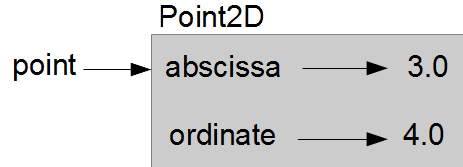
\includegraphics[scale=0.8]{figs/point2D.png}}
\caption{Object diagram.}
\label{fig.point2d}
\end{figure}

The variable {\tt \$point} refers to a {\tt Point2D} object, 
which contains two attributes.  

Each attribute of the {\tt Point2D} class should refer to a 
number, but this is not obvious in the current definition of 
the class. As it stands right now, we could create a {\tt Point2D} 
object with a string for the abscissa, which would not make 
much sense. We can improve the class definition by specifying 
a numeric type for the attributes:
%
\begin{verbatim}
class Point2D {
    has Numeric $.abscissa;              # "x" value
    has Numeric $.ordinate;              # "y" value
}
\end{verbatim}
%
\index{private attribute}
\index{attribute!private}
The instance attributes are private to the class, which means 
that they normally cannot be accessed from outside the class: 
you would usually need to invoke a method of the class 
(i.e. a kind of subroutine defined within the class), to get 
their value. However, when an attribute is defined with a dot 
as in \verb'$.abscissa':

\begin{verbatim}
    has $.abscissa;  
\end{verbatim}
%
\index{accessor}
\index{method!accessor}
Perl automatically creates an implicit \emph{accessor} method, 
i.e. a method having the same name as the attribute and returning  
the value of this attribute. Thus, when we wrote:

\begin{verbatim}
say $point.abscissa;                     # -> 3
\end{verbatim}
%
we were not accessing directly the {\tt abscissa} attribute of 
the \verb'$point' object, but we were really calling the 
{\tt abscissa} method on the object, which in turn returned 
the value of that attribute.

\index{dot notation}
\index{accessor}
You can use such an accessor with dot notation as part of any 
expression. For example:

\begin{verbatim}
my $dist-to-center = sqrt($point.abscissa ** 2 + $point.ordinate ** 2);
\end{verbatim}
%

There is another way to declare an attribute in a class, with 
an exclamation mark instead of a dot:

\begin{verbatim}
    has $!abscissa;  
\end{verbatim}
%
\index{attribute!private}
\index{private attribute}
In that case, Perl does not create an implicit accessor method 
and the attribute can only be accessed from methods within 
the class. Such an attribute is now fully private. 
However, if you declare attributes this way, you 
will not be able to populate them at object creation with 
the default {\tt new} constructor and will need to create your 
own constructor (or indirectly modify {\tt new}). So don't try 
that for the time being, as you would not be able to do much 
with your objects at this point. We'll get back to that later.

\index{attribute!mutable}
\index{attribute!immutable}
By default, object attributes are not mutable, they are read-only. 
This means you cannot modify them once the object has been created. 
This is fine for some attributes: if an object represents a 
person, that person's name and birth date are unlikely to 
change. Some other attributes may need to be updated, sometimes 
very frequently. Attributes can be declared to be mutable 
with the {\tt is rw} trait:
\index{is rw trait}
\index{trait!is rw}

\begin{verbatim}
class Point2D {
    has Numeric $.abscissa is rw;              # "x" value
    has Numeric $.ordinate is rw;              # "y" value
}
\end{verbatim}
%
It is now possible to modify these attributes. For example, 
we can change the newly-created point's abscissa:

\begin{verbatim}
# First creating a Point2D object:
my $point = Point2D.new(abscissa => 3, ordinate => 4);
say $point;    # -> Point2D.new(abscissa => 3, ordinate => 4)

# Now moving the $point object two units to the right:
$point.abscissa = 5; 
say $point;    # -> Point2D.new(abscissa => 5, ordinate => 4)
\end{verbatim}


\index{class attribute}
\index{attribute!class}
Almost all of the above related to instance attributes. You 
can also have attributes pertaining to the whole class, which 
are named \emph{class attributes}. They are less common than 
instance attributes and are declared with the 
{\tt my} declarator (instead of {\tt has}). A typical example 
of a class attribute would be a counter at the class level 
to keep track of the number of objects that have been 
instantiated. 


\section{Creating methods}
\index{method}

The simple {\tt Point2D} class and its instance \verb'$point' 
are not very useful so far. Let's complete the class definition 
with some methods.
\index{Point2D class}

\begin{verbatim}
class Point2D {
    has Numeric $.abscissa;
    has Numeric $.ordinate;
    
    method coordinates {        # accessor to both x and y
        return (self.abscissa, self.ordinate)
    }
    
    method distanceToCenter {
        (self.abscissa ** 2 + self.ordinate ** 2) ** 0.5
    }
    method polarCoordinates {
        my $radius = self.distanceToCenter;
        my $theta = atan2 self.ordinate, self.abscissa;
        return $radius, $theta;
    }
}
\end{verbatim}

We declare three methods in the class:
\begin{itemize}
\item {\tt coordinates}, a simple accessor to the Cartesian 
coordinates;

\item{\tt distanceToCenter}, a method to compute and return 
the distance between the object and the origin;

\index{polar coordinates}
\index{coordinates!polar}
\item{\tt polarCoordinates}, a method to compute the radius 
and azimuth (\verb'$theta') of the object in the polar 
coordinates system (notice that {\tt polarCoordinates} 
invokes the {\tt distanceToCenter} method to find the radius 
component of the polar coordinates).
\end{itemize}

\index{invocant}
A method definition is not very different from a subroutine 
definition, except that it uses the {\tt method} keyword 
instead of the {\tt sub} keyword. This is not a surprise 
since a method is essentially a subroutine that is defined 
within a class (or a role) and knows about its 
\emph{invocant}, i.e. the object that called it and its class. 
And, of course, it has a different calling syntax.
\index{method}

\index{method!dispatch}
\index{dispatching methods}
Another important difference between a subroutine and a method 
is that, since there may be several methods with the same name 
defined in different classes (or different roles), a method 
invocation involves a \emph{dispatch} phase, in 
which the object system selects which method to call, usually 
based on the class or type of the invocant. Except that, in 
Perl~6, that difference is blurred by the fact that you can 
have multi subroutines, i.e. subroutines with the same name 
and a different signature that are also resolved at run time, 
depending on the \emph{arity} (number of arguments) and type of 
the arguments. 
\index{arity}


Within a method definition, {\tt self} refers to the 
\emph{invocant}, the object that invoked the method. 
There is a short hand for it: \verb'$.' so that we could 
write the {\tt coordinates} method as follows:
\index{self}

\begin{verbatim}
    method coordinates {        # accessor to both x and y
        return ($.abscissa, $.ordinate)
    }
\end{verbatim}

The two syntax formats, \verb'$.' and {\tt self.}, are 
essentially equivalent.

There is a third syntactic way of doing it, using an 
exclamation mark instead of a dot:

\begin{verbatim}
    method coordinates {        # accessor to both x and y
        return ($!abscissa, $!ordinate)
    }
\end{verbatim}

Here, the result would be the same, but this new syntax is 
not equivalent: \verb'$.abscissa' is a method invocation, 
whereas \verb'$!abscissa' provides direct access to the attribute.
The difference is that \verb'$!abscissa' is available only 
within the class (and might be slightly faster), while 
the method invocation syntax can be used somewhere else 
(for example in another class). We will see in the next section 
examples of this distinction and its consequences.

We can now create an object and call our methods on it:

\begin{verbatim}
my $point =  Point2D.new(
    abscissa => 4, 
    ordinate => 3
);
say $point.coordinates;         # -> (4 3)
say $point.distanceToCenter;    # -> 5
say $point.polarCoordinates;    # -> (5 0.643501108793284)
\end{verbatim}

\index{topical variable}
\index{invocant}
You might remember from previous chapters that if you use a method 
without naming an explicit invocant, then the method applies to 
the \verb'$_' topical variable:

\begin{verbatim}
.say for <one two three>;       # -> one two three (each on one line)
\end{verbatim}

\index{for loop}
\index{given statement}
Now that we have created an object with some methods, we can also 
take advantage of the same syntax shortcut. For example if we 
use {\tt for} or {\tt given} to populate the \verb'$_' topical 
variable with the \verb'$point' object, we can write:

\begin{verbatim}
given $point {
    say .coordinates;          # -> (4 3)                       
    say .distanceToCenter;     # -> 5                 
    .polarCoordinates.say;     # -> (5 0.643501108793284)
}    
\end{verbatim}

As an exercise, you may write a method called 
\verb"distance_between_points" that takes two Points 
as arguments and returns the distance between
them using the Pythagorean theorem.

The methods of our class so far are all \emph{accessors}, which 
means they provide a snapshot of some of the invocant's attributes. 
If the attributes are mutable (declared with the \verb'is rw' 
trait), we can also create some \emph{mutators}, i.e. methods 
that can be invoked to change those mutable attributes:
\index{accessor}
\index{mutator}

\begin{verbatim}
class Point2D-mutable {
    has Numeric $.abscissa is rw;
    has Numeric $.ordinate is rw;
    
    # perhaps the same accessors as in the class definition above
    
    method new-ordinate (Numeric $ord) {
        self.ordinate = $ord; 
    }
}
# Creating the Point2D-mutable object:
my $point = Point2D-mutable.new(abscissa => 3, ordinate => 4);
say $point;  # -> Point2D-mutable.new(abscissa => 3, ordinate => 4)

# Modifying the ordinate:
$point.new-ordinate(6);
say $point;  # -> Point2D-mutable.new(abscissa => 3, ordinate => 6)
\end{verbatim}




\section{Rectangles and object composition}
\label{rectangles}
\index{rectangle}
\index{composition!object}
\index{object!composition}

Sometimes it is obvious what the attributes of an object should be,
but other times you have to make decisions.  For example, imagine you
are designing a class to represent rectangles.  What attributes would
you use to specify the location and size of a rectangle?  You can
ignore angle; to keep things simple, assume that the rectangle is
either vertical or horizontal.
\index{representation}

There are at least two possibilities: 

\begin{itemize}

\item You could specify one corner of the rectangle
(or the center), the width, and the height.

\item You could specify two opposing corners.

\end{itemize}

At this point it is hard to say whether either is better than
the other, so we'll implement the first one, just as an example.
\index{Rectangle class}
\index{class!Rectangle}

Here is the class definition:

\begin{verbatim}
class Rectangle {
    has Numeric $.width;
    has Numeric $.height;
    has Point2D $.corner;     # lower left vertex 

    method area { return $.width * $.height }
    method topLeft { $.corner.abscissa, $.corner.ordinate + $.height; }
    # other methods, e.g. for other corners' coordinates, center, etc.
}
\end{verbatim}
%
The new feature compared to the previous {\tt Point2D} class 
definition is that the \verb'Rectangle' class can now use the 
{\tt Point2D} type created previously for defining the corner 
attribute. 

The {\tt topLeft} method returns the coordinates of 
the top left angle of the rectangle. This {\tt topLeft} 
method is an opportunity to explain a bit more 
the difference between the \verb'$.' and \verb'$!' twigils. We have 
used \verb'$.corner.abscissa' to access to the abscissa of 
the corner, i.e. in effect two accessor invocations. We could 
have accessed directly to the {\tt corner} and {\tt height} 
attributes of the {\tt Rectangle} class and used the following 
method definition:

\begin{verbatim}
    method topLeft { $!corner.abscissa, $!corner.ordinate + $!height; }
\end{verbatim}

But it would not be possible to use \verb'$!corner!abscissa' or 
\verb'$.corner!abscissa', because {\tt abscissa} is not an 
attribute defined in the {\tt Rectangle} class, and thus cannot 
be accessed directly there. You can use direct access 
to the attribute (for example with the \verb'$!abscissa' syntax) 
only within the class where this attribute is defined, 
{\tt Point2D}. So, in {\tt Rectangle}, we need to invoke the 
accessor (i.e. the syntax with \verb'$.') for obtaining the 
value of the corner abscissa.

We can now create a {\tt Rectangle} object:
\index{rectangle}

\begin{verbatim}
my $start-pt =  Point2D.new(abscissa => 4, ordinate => 3);
my $rect = Rectangle.new(corner => $start-pt, height => 10, width => 5);

say "Topleft coord.: ", $rect.topLeft;   # -> Topleft coord.: (4 13)
say "Rectangle area: ", $rect.area;      # -> Rectangle area: 50
\end{verbatim}

\index{named parameter}
\index{parameter!named}
You might have noticed that the arguments passed to the 
{\tt Rectangle.new} constructor are not in the same order as 
in the class definition. We did that on purpose 
to show that the order is unimportant because we 
are using named arguments.


\begin{figure}
\centerline
{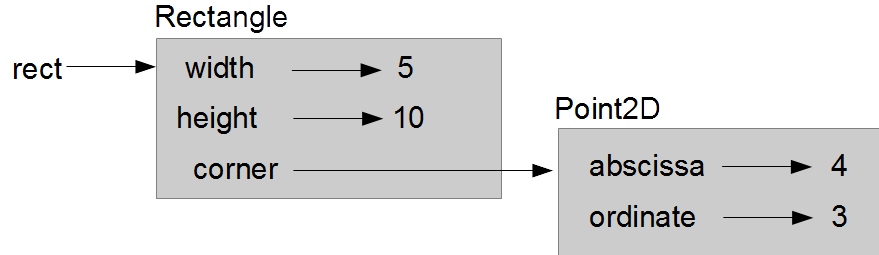
\includegraphics[scale=0.8]{figs/rectangle.png}}
\caption{Object diagram.}
\label{fig.rectangle}
\end{figure}


Figure~\ref{fig.rectangle} shows the state of this object.

\index{state diagram}
\index{diagram!state}
\index{object diagram}
\index{diagram!object}
\index{embedded object}
\index{object!embedded}
\index{object!composition}
\index{composition!object}

Using an object as an attribute of another object, possibly 
of another class, is called {\bf object composition}. An object 
that is an attribute of another object is {\bf embedded}. Object 
composition makes it possible to easily define nested layers of 
abstraction and is a powerful feature of object oriented 
programming. In our ``geometry'', we started to define a low 
level object, a {\tt Point2D} instance, and then used that point 
to define a higher level type, {\tt Rectangle}.


\section{Instances as return values}
\index{instance!as return value}
\index{return!value}

Methods can return instances of another class.  For example, 
the {\tt Rectangle} class can have methods returning 
instances of {\tt Point2D} for the other corners:

\begin{verbatim}
    method topRightPoint {
        return Point2D.new(
            abscissa => $!corner.abscissa + $!width, 
            ordinate => $!corner.ordinate + $!height
        );
    }
   # other methods for other corners
\end{verbatim}

Notice that we don't even bother to give a name to upper right 
point (although we could, if we wanted); we create it with the 
constructor and return it on the fly.

We can use the new method as follows:

\begin{verbatim}
my $topRightPt = $rect.topRightPoint;
say "Top right corner: ", $topRightPt;
# -> Top right corner: Point2D.new(abscissa => 9, ordinate => 13)
\end{verbatim}

\index{type}
Although this is not very useful in such a simple case, we 
could play it safe and declare a {\tt Point2D} type for 
\verb'$topRightPt':

\begin{verbatim}
my Point2D $topRightPt = $rect.topRightPoint;
\end{verbatim} 

This way, the code will raise an error if the {\tt topRightPoint} 
happens to return something else than a {\tt Point2D} instance.

Similarly, the \verb"find-center" method invoked on a 
{\tt Rectangle} returns a {\tt Point2D} instance 
representing the center of the {\tt Rectangle}:

\begin{verbatim}
    method find-center { Point2D.new(
            abscissa => $!corner.abscissa + $!width / 2, 
            ordinate => $!corner.ordinate + $!height / 2
        );
    }
\end{verbatim}
%
This new method can be used as follows:

\begin{verbatim}
say "Center = ", $rect.find-center;
# -> Center = Point2D.new(abscissa => 6.5, ordinate => 8.0)
\end{verbatim}
%

\section{Inheritance}
\index{inheritance}
\index{inheritance!class}
\index{class inheritance}


Inheritance is probably the most emblematic feature of 
object-oriented programming. It is a mechanism through which it 
is possible to derive a class from another class. Inheritance is 
one of the standard ways to implement code reuse in 
object-oriented programming. It is also another useful way of 
defining successive layers of abstraction and a hierarchy of 
types.

\subsection{The Pixel class}
\index{class!Pixel}
\index{Pixel class}

The {\tt Point2D} class is very general and could be used for 
a variety of purposes: geometry, vector graphics, animated mangas 
and so on. We may want to use it to display graphic data on a 
screen. For this, we may want to create a new derived class, 
{\tt Pixel}, adding new properties to the point, such as color, 
perhaps transparency, etc. 

Do we need to redefine all the attributes and methods for 
the new class? No, we don't. We can define a new class that 
\emph{inherits} the properties of the {\tt Point2D} base class 
and only modify what is no longer suitable or add whatever 
new features we need. Here, we want a new attribute to represent 
the pixel color and probably some new methods dealing with this 
new attribute.

According to the most common standards, a color is defined 
by three integers (really three octets, i.e. integers 
between 0 and 255 in decimal notation), representing the red, 
green and blue (RGB) components of the pixel:
\index{class!child}
\index{pixel class}
\index{RGB}

\begin{verbatim}
class Pixel is Point2D {
    has %.color is rw;

    method change_color(%hue) {
        self!color = %hue
    }
    method change_color2(Int $red, Int $green, Int $blue) {
        # signature using positional parameters
        self!color = (red => $red, green => $green, blue => $blue)
    }
}
\end{verbatim}

\index{parameter!positional}
\index{parameter!named}
\index{positional parameter}
\index{octet}
\index{is!subclassing trait}
The new class \emph{inherits} the properties of {\tt Point2D} 
thanks to the {\tt is Point2D} trait, except possibly those 
which are explicitly modified (or overridden) or added in 
the new class. The new class is sometimes 
called child class or subclass, whereas {\tt Point2D} is the 
parent class. Creating this new class based on 
{\tt Point2D} is called subclassing the {\tt Point2D} 
parent class. 
\index{class!parent}
\index{class!child}
\index{class!subclass}
\index{subclassing}
\index{overriding a method}
\index{method!overriding}

The new child class inherits the {\tt abscissa} and 
{\tt ordinate} attributes of the {\tt Point2D} parent 
class (and their specific type and properties if any), 
as well as the methods such as {\tt coordinates} defined 
in the parent class. The child class  has a new 
attribute (the color) and two new methods.

We have written here two different methods for changing the color 
only to illustrate two possible syntax formats, for pedagogical 
purpose. The first one receives a hash as a parameter, and 
the second one uses positional parameters, which forces 
the user to remember the order (RGB) in which the arguments must 
be passed; this can be a source of error and should be avoided 
when the number of the parameters exceeds a certain limit 
(which will be left to the decision of the reader). On the other 
hand, anyone working commonly with graphics knows by heart the 
standard conventional order of colors (i.e. RGB). Also, 
the second method has the 
advantage of enabling some type checks (the arguments must 
be integers). This is a simplified example; in real life, it 
may be desirable to check that the parameters are octets, i.e. 
integers between 0 and 255 (which could be done by adding a 
type constraint or defining a subset of the Integer type).
\index{subset}
\index{RGB}
\index{octet}

Using the new {\tt Pixel} class is straight forward:

\begin{verbatim}
say "Original colors: ", $pix.color;

$pix.change_color({:red(195), :green(110), :blue(70),});
say "Modified colors: ", $pix.color;
say "New pixel caracteristics:";
printf \tAbscissa: %.2f\n\tOrdinate: %.2f\n\tColors: R: %d, G: %d, B: %d\n",
       $pix.abscissa, $pix.ordinate, 
       $pix.color<red>, $pix.color{"green"}, $pix.color{"blue"};

$pix.change_color2(90, 180, 30);  # positional args
say "New colors:  R: {$pix.color<red>}, G: {$pix.color<green>}, B: {$pix.color<blue>} ";
\end{verbatim}

This displays the following output:

\begin{verbatim}
Original colors: {blue => 145, green => 233, red => 34}
Modified colors: {blue => 70, green => 110, red => 195}
New pixel caracteristics:
        Abscissa: 3.30
        Ordinate: 4.20
        Colors: R: 195, G: 110, B: 70
New colors:  R: 90, G: 180, B: 30
\end{verbatim}

To tell the truth, it was not necessary to use two different 
method names, \verb'change_color' and \verb'change_color2', as 
we did in the {\tt Pixel} class definition. It would just 
work the same way if we use these definitions:
\index{pixel class}
\index{method dispatch}

\begin{verbatim}
    multi method change_color(%hue) {
        self.color = %hue
    }
    multi method change_color(Int $red, Int $green, Int $blue) {
        # signature using positional parameters
        self.color = (red => $red, green => $green, blue => $blue)
    }
\end{verbatim} 

Since the multi method is defined twice, with the same name but 
with a different signature, the object system is able to 
dispatch the invocation to the right method.
\index{method!dispatch}
\index{multi method}


\subsection{The MovablePoint class}
\index{class!MovablePoint}
\index{MovablePoint class}

The \verb'$.abscissa' and \verb'$.ordinate' attributes of 
class {\tt Point2D} are defaulted to read-only. After all, 
when you define a point in the plan, it usually has a fixed 
position and there is generally no reason to change its 
coordinates.

Suppose, however, that our application is about kinematics 
(the branch of physics dealing with the motion of points or 
bodies) or is a video game. In such a case, we probably want 
our points (or sets of points) to move. We need a new class, 
{\tt MovablePoint}, enabling the modification of coordinates.

We don't need to redefine all the attributes and methods for 
the new class. We can define a new class that 
\emph{inherits} the properties of the {\tt Point2D} base class 
and only modify what is no longer suitable or add whatever 
new features we need, for example:

\begin{verbatim}
class MovablePoint is Point2D {
    has Numeric $.abscissa is rw;
    has Numeric $.ordinate is rw;
    
    method move (Numeric $x, Numeric $y) {
        $.abscissa += $x;
        $.ordinate += $y;
    }
}
\end{verbatim}

\index{is!subclassing trait}
Again, the new class inherits the properties of {\tt Point2D} thanks 
to the {\tt is Point2D} trait, except those which are explicitly 
modified (or overridden) or added in the new class. 
Methods that exist in the parent class and are 
redefined in a child class are said to be \emph{overridden} 
within that class. 
\index{class!parent}
\index{class!child}
\index{class!subclass}
\index{subclassing}
\index{overriding a method}
\index{method!overriding}

Here, the \verb'$.abscissa' and \verb'$.ordinate' attributes are 
redefined as read and write (through the {\tt is rw} trait) and 
a new method, {\tt move}, is defined to modify the position of 
a point by adding the received parameters to the coordinates 
of the point.
\index{is rw trait}

Note that we have used here positional parameters for the 
{\tt move} method. We said that it is often better for the sake of clarity 
to use named parameters, but we have here only two parameters, 
and, as it is fairly simple to remember that the \verb'$x' 
parameter should come before the \verb'$y' parameter, this 
was a good occasion to illustrate this possibility.
\index{positional parameter}
\index{parameter!positional}
\index{parameter!named}
\index{named parameter}

We can now test our new child class, create a {\tt MovablePoint} 
instance, display its characteristics, move it to a different 
location, and display the new position:

\begin{verbatim}
my $point = MovablePoint.new(
    abscissa => 6,
    ordinate => 7,
    );

say "Coordinates : ", $point.coordinates;
say "Distance to origin: ", $point.distanceToCenter.round(0.01);
printf "%s: radius = %.4f, theta (rad) = %.4f\n", 
    "Polar coordinates", $point.polarCoordinates;

say "--> Moving the point.";
$point.move(4, 5);
say "New coordinates: ", $point.coordinates;
say "Distance to origin: ", $point.distanceToCenter.round(0.01);
printf "%s: radius = %.4f, theta (rad) = %.4f\n", 
    "Polar coordinates", $point.polarCoordinates;
\end{verbatim}

This produces the following output:

\begin{verbatim}
Coordinates : (6 7)
Distance to origin: 9.22
Polar coordinates: radius = 9.2195, theta (rad) = 0.8622
--> Moving the point.
New coordinates: (10 12)
Distance to origin: 15.62
Polar coordinates: radius = 15.6205, theta (rad) = 0.8761
\end{verbatim}

\index{polar coordinates}
\index{coordinates!polar}
Here, when the user code invokes the {\tt coordinates}, 
{\tt distanceToCenter} and {\tt polarCoordinates} methods, 
Perl find that they do not exist in {\tt MovablePoint}. But, 
as \verb'MovablePoint' subclasses {\tt Point2D}, the program 
looks for method having this name in the parent class and 
invokes them if it finds them. 	If it did not find them, it 
might look up into the parent's parent if there is any, and 
so on.


\subsection{Multiple inheritance: attractive, but is it wise?}

In object-oriented programming, the inheritance mechanism is 
a traditional way to reuse code, it is even probably the most 
common way to do it. 

A class may have several parent classes and, thus, subclass 
several other classes. This is what is called multiple 
inheritance. We might want to build a new {\tt MovablePixel} 
class inheriting from both {\tt MovablePoint} and {\tt Pixel} 
(and, indirectly, from {\tt Point2D}). Technically, you can 
easily do it in Perl:

\begin{verbatim}
class MovablePixel is MovablePoint is Pixel {
    # ...
}
\end{verbatim}

Now, {\tt MovablePixel} is subclassing both 
{\tt MovablePoint} and {\tt Pixel} and inheriting 
from both parent classes.
\index{subclass}
\index{class!parent}

This looks very promising, but it turns out to be more 
complicated than expected in real situations. If there is a 
conflict (for example a name collision between two methods), 
which one shall prevail? There exists some mechanism to 
handle such situations (for example in the C++ programming 
language), and Perl has some metaobject methods to find out 
about the method resolution order (MRO), but this 
might quickly leads to severe design 
problems and to really subtle or complicated bugs. In 
short, while multiple inheritance originally looked as a 
attractive idea, it turned out to be complicated to master, 
because it creates multiple and often implicit dependencies 
that are quite hard to sort out.

This is the reason why, contrary to C++, relatively more recent 
OO programming languages such as Java (which came out not 
so recently, back in 1995) have decided not to implement 
multiple inheritance.

Perl~6 does not want to forbid such things and allows you 
to do multiple inheritance if you wish, and it can be useful 
for simple cases; so don't necessarily rule it out, but, 
contrary to early expectations, it often leads to a mess and
turns out to be quite unmanageable.

Perl offers better concepts for tackling such situations,
as we will see shortly.

\section{Roles and composition}
\index{role}
\index{inheritance}

Inheritance is a very powerful concept to describe a hierarchical 
tree of concepts. For example, you can think of a hierarchy of 
geometrical figures having more and more specific properties: 
\begin{enumerate}
\item Polygon.

\index{quadrilateral}
\item Quadrilateral (a polygon with four edges and four corners).

\index{trapezoid}
\item Trapezoid (a quadrilateral with one pair of parallel edges).

\index{parallelogram}
\item Parallelogram (a trapezoid with two pairs of parallel 
edges and opposite sides of equal length).

\index{rectangle}
\item Rectangle (a parallelogram with four right angles).

\index{square}
\item Square (a rectangle with all four sides of equal length).
\end{enumerate}

\index{rhombus}
It is relatively easy to imagine a series of classes with a 
hierarchical inheritance tree reflecting those properties. It 
gets slightly more complicated, however, if we add the rhombus 
(a parallelogram with all sides equal), because the square is 
now \emph{also} a rhombus with four right angles, so that 
the square class would subclass both the rectangle and the 
rhombus, and we might have here a possible multiple inheritance 
issue.

\index{integer} \index{rational} \index{real number} \index{complex number}
\index{vertebrate} \index{mammal} \index{carnivoran}
\index{canid} \index{dog}
Similarly, we can think of a tree of classes with nested 
inheritance representing various types of numbers (e.g. integer, 
rational, real, complex) or animals species (e.g. vertebrate, 
mammal, carnivoran, canid, dog, Irish setter).

\index{hierarchical model}
These are great examples for inheritance, but the real world is 
rarely so hierarchical, and it is often difficult to force 
everything to fit into such a hierarchical model.

\index{role}
This is one of the reasons why Perl introduces the notion of 
roles. A role is a set of behaviors or actions that can be shared 
between various classes. Technically, a role is a collection 
of methods (with possibly some attributes); it is therefore 
quite similar to a class, but the first obvious difference 
is that a role is not designed to be instantiated as an object 
(although roles can be promoted into classes). The 
second difference, perhaps more important, is that roles 
don't inherit: they are used through application to a class 
and/or composition.

\subsection{A mammal class and a pet-animal role}

\index{vertebrate} \index{mammal} \index{dog}
Let's come back to vertebrates, mammals and dogs. A dog is 
a mammal and inherits some characteristics from the mammals, 
such as having a neocortex (a region of the brain), hair, 
and mammary glands, as well as a vertebral column, which 
all mammals (along with fishes, birds, reptiles and others) 
inherit from vertebrates. So far, the class hierarchy seems 
simple and natural.

\index{feral animal}
\index{pet animal}
But dogs can have very different characteristics and behaviors.
To quote the Wikipedia article on dogs: ``Dogs perform many 
\emph{roles} for people, such as hunting, herding, pulling 
loads, protection, assisting police and military, companionship 
and, more recently, aiding handicapped individuals'' (italic emphasis 
added). Dogs can also be \emph{feral} animals 
(i.e. animals living in the wild but 
descended from domesticated individuals) or stray dogs. All 
these additional behaviors might be added to the dog class. 
Similarly, a cat, another mammal, may also be a pet 
or a feral animal. Mustangs, North-American free-roaming horses, 
are also feral animals, descending from once-domesticated horses; 
but a mustang may also be captured and brought back to 
domesticated state. This return to the wild of feral animals 
is not limited to mammals: pigeons living in our cities are 
often descending from once-domesticated homing pigeons used 
in the past. It can even happen with invertebrates, such 
as swarms of honey bees.

It is apparent that a hierarchical modeling of inheritance 
trees is not adapted to describe such behaviors. 

\index{vertebrate} \index{mammal} \index{dog}
We can define classes for dogs, cats, and horses as subclasses 
of mammals (which itself inherits from vertebrates). Besides 
that, we define roles for pet or feral animals. In addition, 
we can create new classes subclassing the dog, horse and cat 
classes and doing some specific roles; or we can assign roles 
to individual instances of a class. This could look like this 
(this is a dummy example which cannot be tested):

\begin{verbatim}
class Vertebrate { method speak {say "vertebrate"};}
class Mammal  is Vertebrate  { method speak { say "mammal" } }
class Bird    is Vertebrate  { method fly    {} }
class Dog     is Mammal      { method bark   {} }
class Horse   is Mammal      { method neigh  {} }
class Cat     is Mammal      { method meow   {} }
class Mouse   is Mammal      { method squeek {} }
class Duck    is Bird        { method quack  {} }
# ...

role Pet-animal { 
    method is-companion() {...} 
    # other methods
}
role Shepherd   { ... }    # sheep keeper
role Feral      { ... }    # animal back to wild life
role Guide      { ... }    # blind guide
role Human-like { ... }    # animal behaving like a human
# ...

class Guide-dog        is Dog    does Guide      { ... }
class Shepherd-dog     is Dog    does Shepherd   { ... }
class Stray-dog        is Dog    does Feral      { ... }
class Pet-cat          is Cat    does Pet-animal { ... }
class Feral-cat        is Cat    does Feral      { ... }
class Mustang          is Horse  does Feral      { ... }
class Domestic-canary  is Bird   does Pet-animal { ... }
# ...
# Role can also be applied to instances:
my $garfield = Pet-cat.new(...);
my $mickey   = Mouse.new(...);
$mickey does Human-like;
my $donald   = Duck.new(...);
$donald does Human-like;
my $pluto    = Dog.new(...);
$pluto does Pet-animal;
my $snoopy   = Dog.new(...);
$snoopy does Pet-animal does Human-like;
\end{verbatim}
 
\index{role!application}
\index{does trait}
\index{trait!does}
\index{trait!is}
A role is applied to a class or an object with the {\tt does} 
trait (as opposed to {\tt is} for inheritance). These 
different keywords reflect the semantic difference associated 
to them: composing a role into a class or an object provides 
this class or object with the \emph{supplementary behavior} associated with 
the role, but it does not follow that the object receiving 
the role is \emph{the same thing} as or of the same nature 
as the role.

\index{feral animal}
\index{pet animal}
If the {\tt Pet-animal} and {\tt feral} roles had been defined 
as classes, then the {\tt Pet-cat} and {\tt Feral-cat} classes 
would have undergone double inheritance, with the potential 
problems associated with that. By applying a role to a 
class, you avoid constructing a multiple-inheritance tree 
that is probably not really justified and can be complicated 
to conceptualize and difficult to maintain. Judicious use 
of classes and roles can lead to a model that is simpler, 
more natural, and closer to the real relations between the 
entities and behaviors under scrutiny.

\index{multiple inheritance}
\index{method!dispatch}
\index{role!composition}

In addition, if you inadvertently compose several roles with 
two methods having the same name, this raises immediately 
an error (unless a method of the same name exists within the 
class, in which case it prevails), rather than dispatching 
silently to one of the two methods as in the case of multiple 
inheritance. In that case, naming conflicts are identified 
immediately (at compile time), which has the benefit of 
immediately finding a bug that might otherwise go 
unseen for a while.

\subsection{Role composition and code reuse}

Classes are meant for managing instances and roles are 
meant for managing behaviors and code reuse.
\index{class}
\index{role}
\index{code reuse}

\begin{verbatim}
role Drawable {
    has $.color is rw;
    method draw { ... }
}
class Figure {
    method area { ... }
}
class Rectangle is Figure does Drawable {
    has $.width;
    has $.height;
    method area {
        $!width * $!height;
   }
    method draw() {
        for 1..$.height {
            say 'x' x $.width;
        }
    }
}
Rectangle.new(width => 10, height => 4).draw;
\end{verbatim}

\index{ellipsis}
Please note that the ellipsis \verb'...' used in the code 
above is really meant here to represent some code that is left 
to your implementation. However, this is actually valid code 
and it will compile and even run without any problem. The 
ellipsis is used to figure a functionality that is not yet 
there but is supposed to be implemented at a later point. This 
will work so long as you don't invoke these methods (you would 
get a runtime error) or don't setup a situation where it would 
need to be defined (which would cause a compile time error. 
In the case of the {\tt draw} method in the 
{\tt Drawable} role, role composition into the {\tt Rectangle} 
class works only because {\tt draw} is redefined in the 
{\tt Rectangle} class; without this redefinition, it would 
have raised a compile-time error. Similarly, 
the \verb'method area { ... }' 
code of the {\tt Figure} class would raise a run-time error if it 
were called without having been redefined in the {\tt Rectangle} 
class. The ellipsis has been used here only as a convenient way 
to represent code whose implementation is not important for 
our example because it is being redefined anyway. In real coding, 
it is probably best advised not to use it except as an expedient 
for code that is not yet developed but will be really implemented.

This draws an ASCII rectangle:
\begin{verbatim}
~ perl6 test_drawable.pl6
xxxxxxxxxx
xxxxxxxxxx
xxxxxxxxxx
xxxxxxxxxx
\end{verbatim}

\subsection{Roles, classes, objects, and types}
\index{role}
\index{class}
\index{object}
\index{type}

A role can be applied to an entire class or only to some 
instances of the class:

\begin{verbatim}
role Guide { ...}
class Guide-dog is Dog does Guide { 
    ... 
}  # Composing the Guide role into the Guide-dog class
   # inheriting from the Dog class

my $doggy = new Dog;    # creating a Dog object
$doggy does Guide;      # applying the role to the object
\end{verbatim}

\index{type}
\index{role!type}
\index{type!-defining role}
\index{guide}
Roles and classes are different, but both are or define types.
This means that a role can be used as a type for a variable 
declaration where you might expect a class name. For example, 
the {\tt Guide} role sketched in the code snippet above does 
effectively create a {\tt Guide} type. So a {\tt Blind} role for 
a human might have an attribute of {\tt Guide} type, which 
might represent a guide-doq, a guide-horse, a human guide or 
even a guiding robot.

\begin{verbatim}
class Human {
    has Dog $dog;      # May contain any dog, with or without
                       # a guide role
}
role Blind {
    has Guide $guide;  # May contain any Guide type, whether 
                       # a dog, a horse, a human or a robot
}
\end{verbatim}

\index{type!built-in}
A number of Perl~6 built-in types are defined by roles and 
not by classes, such as {\tt IO}, {\tt Iterable}, 
{\tt Iterator}, {\tt Numeric}, {\tt Rational}, {\tt Real},
etc.

\section{Method delegation}
\index{delegation}

Delegation is another way to link an object to another piece 
of code. The delegation technique has been relatively well 
studied at the theoretical level and implemented in a few 
specialized research languages, but mainstream generalist 
languages implementing delegation are rather rare.

Rather than defining methods in a class or in a role, the 
idea is to invoke methods belonging to another object, as 
if they were methods of the current class. In Perl~6, delegation 
may be performed at the level of a class or a role. A delegated 
object is simply an attribute defined in the class or in the role 
with the {\tt handles} keyword which makes it possible to specify 
which methods of the delegated object may be used in the 
current class.

\index{Cervantes, Miguel de} \index{Shakespeare, William} 
\index{Chekhov, Anton} \index{Schiller, Friedrich} \index{Hamlet} 
\index{Don-Quijote} \index{Don-Carlos} \index{Three Sisters}
\begin{verbatim}
class BaseClass {
    method Don-Quijote()    { "Cervantes"   }
    method Hamlet()         { "Shakespeare" }
    method Three-Sisters () { "Chekhov"     }
    method Don-Carlos()     { "Schiller"    }
}
class Uses { 
    has $.base is rw handles < Don-Quijote Hamlet Three-Sisters >;
}

my $user = Uses.new;
$user.base = BaseClass.new(); # implementing an object-handler
say $user.Don-Quijote;
say $user.Hamlet;
say $user.Three-Sisters;
say $user.Don-Carlos;
\end{verbatim}

This displays the following output:

\begin{verbatim}
Cervantes
Shakespeare
Chekhov
Method 'Don-Carlos' not found for invocant of class 'Uses'
  in block <unit> at delegate.pl6 line 16
\end{verbatim}

The program properly displays the names of writers returned 
by the first three methods, because they have been sort of 
``imported'' into the {\tt Uses} class, but it fails on the 
last one, because ``Don-Carlos'' is not part of the handler's 
list. The error on the last method is a run-time exception 
and the program would stop running there even if there 
were some more correct code afterward. 

Note that the {\tt Uses} class does not know from where the 
methods will be imported; it only knows about the names of 
the methods that will be imported. It is only when the 
\verb'$user' object is created and the \verb'$user.base' 
attribute added to it that the methods defined in {\tt BaseClass} 
that the object is dynamically associated with these methods. 
By the way, this process could be done in just one step:

\begin{verbatim}
my $user = Uses.new( base => BaseClass.new() );
\end{verbatim}

There is no need to enumerate the methods to be handled. The 
{\tt Uses} class can import all the methods of {\tt BaseClass}:

\begin{verbatim}
class Uses { 
    has $.base is rw handles BaseClass;
}
\end{verbatim}

This will work as before, except of course that it will not fail 
on the {\tt Don-Carlos} method this time, since this method is 
also imported now:

\begin{verbatim}
Cervantes
Shakespeare
Chekhov
Schiller
\end{verbatim} 

\section{Polymorphism}
\index{polymorphism}
\index{interface}

Polymorphism is a way to supply a common or close interface 
to different types. In a certain way, the inheritance examples 
studies previously offer a form of polymorphism: the 
{\tt coordinates}, {\tt distanceToCenter} and {\tt PolarCoordinates} 
methods are polymorphic, since they can apply to 
{\tt Point2D}, {\tt movablePoint} and {\tt pixel} types. But 
these are trivial forms of polymorphism. We will speak of 
polymorphism when the relevant methods or functions are 
doing something different, at least at the implementation 
level, even if they share the same name and interface.

\index{multi!subroutine}
Outside of the object-oriented programming, Perl's 
\emph{multi} subroutines implement a form of polymorphism, 
since they can do something very different according to the 
type and number of their arguments. Within the OOP context, 
it is often the type of the invocant (its class or possibly one 
of its roles) which will determine, usually at run-time, 
which of the possible methods will be invoked.

For example, we might want to create a new class for points 
in a three-dimensional space. The methods will have to be 
different, but it seems interesting to offer the user an 
interface that is the same (or almost) as for two-dimensional 
points.  
\index{Point3D class}

\begin{verbatim}
class Point3D {
    has Numeric $.x;
    has Numeric $.y;
    has Numeric $.z;
    
    method coordinates () {      # accessor to the 3 coordinates
        return $.x, $.y, $.z
    }
    method distanceToCenter () {
        return ($.x ** 2 + $.y ** 2 + $.z ** 2) ** 0.5
    }
    method polarCoordinates () {
    	return self.sphericalCordinates;
    }
    method sphericalCoordinates {
    	my $rho = $.distanceToCenter;
    	my $longitude = atan2 $.y, $.x;          # theta
    	my $latitude = acos $.z / $rho;          # phi 
    	return $rho, $longitude, $latitude;
    }
    method cylindricalCoordinates {
    	# ...
    }
}
\end{verbatim}

The methods in this new class are not the same as those in 
{\tt Point2D}, but methods having a similar semantics have 
the same name; it is thus possible to use either class 
without being lost with different names. 

The {\tt distanceToCenter} method has exactly the same interface. 
The {\tt coordinates} method returns a list of three values 
instead of two, but the calling convention is the same. Note 
that it might also have been possible to design {\tt Point2D} 
so that this method would also a third zero value, in order 
to have exactly the same interface (after all, a point in 
the plane might be considered as a point in the 3D space 
with a zero height); complying to exactly the same 
interface is not mandatory, but only a possible implementation 
decision that might make a more intuitive interface. 

\index{polar coordinates}
\index{spherical coordinates}
\index{coordinates!polar}
\index{coordinates!spherical}
The notion of polar coordinates does not have a well-defined 
meaning in a 3D-space, but we have chosen here to keep the name 
in our interface because it is intuitively quite similar to 
the idea of spherical coordinates; but it does nothing more 
than invoking the sphericalCoordinates method on its invocant 
and to return the return values.

Please note that mathematicians, physicists, astronomers, 
engineers, geographers, and navigators all use the same basic system 
for spherical coordinates, but their conventions are different 
concerning the origin, the angle range, angle measurement 
units and rotation direction, and the name of the various 
values or symbols associated with them. So you might find 
some different formulas in a textbook. The conventions and 
formulas we have used here are commonly used in geography and 
some branches of mathematics. A real general-purpose class 
might have to take these varying conventions into account and 
implement the necessary conversions.

\section{Encapsulation}

\index{encapsulation}
Encapsulation is the idea of hiding the data and the code 
of a library or a module from the user. It is not specific to 
object-oriented programming, but it is a fundamental concept 
of OOP.

\index{accessor}
\index{mutator}
\index{getter}
\index{setter}
In object-orienting programming, encapsulation consists in 
protecting the data in an object from being tampered 
directly (and possibly made inconsistent) 
by their user, who can access such data only through
the means of methods. This is achieved by providing to the 
user methods that are commonly called \emph{accessors} (or 
\emph{getters}) and \emph{mutators} (or \emph{setters}). This 
makes is possible to ensure that the object properties will 
be validated by its methods.

\index{black box}
\index{object!interface}
Encapsulation is a strong form of data abstraction and 
procedural abstraction. Seen from outside, an object 
is a black box having some specified properties and 
behaviors. This way, these properties and behaviors are 
\emph{hidden} from the user. They're not hidden in the 
sense that the user cannot know about them (at least in 
the open-source world, it is easy to know that), but it 
is hidden in the sense that it is usually not possible to 
use that knowledge to bypass the supplied interface. This 
means that the internal implementation of the object may 
change without modifying the external behavior. If you 
are going to use insider knowledge, your code will 
probably break when the internal implementation is 
modified, so don't do that.

Various programming languages don't have same rules for 
guaranteeing encapsulation, some are stricter than others, 
some are less restrictive for read access than for write access, 
others don't make such a distinction but rather rely on the 
visibility level specified for an attribute, for example 
``public'' or ``private'' (with sometimes an intermediate 
``protected'' level).

\index{attribute!private}
Perl~6 lets you choose the encapsulation model you want to 
apply to your objects and attributes. All attributes are 
private. If you declare a class as follows:

\begin{verbatim}
class Point2D {
    has $!abscissa;
    has $!ordinate;
    # …
    method value_x { return $!abscissa }
    method value_y { return $!ordinate }
}
\end{verbatim}

the \verb'$!x' and \verb'$!y' coordinates will be 
accessible only from within the class. This is why 
we have added accessor methods. In addition, the 
attributes are immutable by default.

But as we have seen earlier, if you declare this class 
as follows:

\begin{verbatim}
class Point2D {
    has $.abscissa;
    has $.ordinate;
    # ...
}
\end{verbatim}

the coordinates will still be private attributes, but Perl~6 
will automatically generate accessor methods having the same 
names as the attributes, so that it will be possible to access 
them from outside the class almost as if they were public:
\index{attribute!public}

\begin{verbatim}
class Point2D {
    # ...
}
my $point = Point2D.new(abscissa => 2, ordinate => 3);
say $point.abscissa;       # -> 2
\end{verbatim}

\index{attribute!mutable}
\index{attribute!immutable}
Whether the attribute is mutable or not is managed separately 
by the {\tt is rw} trait. In brief, Perl~6 offers a default 
access mode, but you can finely tune what you need.


\subsection{Private methods}
\index{private method}
\index{method!private}
\index{interface}

Methods are the normal way to use objects, whether with read only 
or read and write access. They usually form the \emph{interface} 
of a class, that is the part of the class that is made public 
and available to programmers wishing to use them. It is thus 
natural and legitimate for methods to be public, i.e. accessible 
from outside the class.
\index{method!public}
\index{public method}

But a class may also contain numerous methods that are part 
of the internal cooking recipes of the class and that are not 
meant to be used from outside the class. It is possible to prevent 
their use from outside the class by making these methods private. 
A Perl~6 private method is prefixed with an exclamation mark:

\begin{verbatim}
method !private-behavior($x, $y) {
    ...
}
\end{verbatim}

You will also need to use an exclamation mark to call them:

\begin{verbatim}
$my-object!private-behavior($val1, $val2)
\end{verbatim}

\index{private method}
\index{method!private}
Private methods are really internal to a given class. In 
particular, they are not inherited by child classes.


\subsection{Constructing objects with private attributes}

Constructing objects with private attributes raises a 
little difficulty. Let's consider the following program:
\index{private attribute}

\begin{verbatim}
class Point3D {
    has $.x;
    has $.y;
    has $!z;
    
    method get {
        return ($!x, $!y, $!z);
    }
};

my $a = Point3D.new(x => 23, y => 42, z => 2);
say $_ for $a.get;
\end{verbatim}

\index{attribute!private}
\index{attribute!public}
In this example, we have declared \verb'$.x' and \verb'$.y' 
as ``public'' (so to speak) attributes, and \verb'$.z' as 
a truly private attribute. Running this code displays this:

\begin{verbatim}
23
42
(Any)
\end{verbatim}

Oops, what is going on? It seems that the {\tt get} 
method is not able to read \verb'$!z', since it returns 
an undefined value. This method is defined within the 
class; so it should be able to access this attribute. In 
fact, {\tt get} is not guilty, it is \verb'$!z' which is 
not defined within the object, because it hasn't been properly 
initialized during object construction.

\index{new!constructor}
\index{constructor!new}
The guilt lies with the {\tt new} implicit constructor which, 
by default, initializes only ``public'' attributes.

\index{submethod}
Here, the simplest solution is probably to add a {\tt BUILD} 
submethod in the class definition.
\index{BUILD submethod}

\index{submethod}
\index{subclass}
\index{type}
A \emph{submethod} is a public method that is not inherited 
in child class. Semantically, it is really equivalent 
to a subroutine, but it is called with a method syntax (hence 
the name). Submethods are especially useful to perform object 
construction and destruction tasks which should not be 
inherited by subclasses, as well as for tasks that are 
so specific to a given type that classes derived from it  
will almost for sure have to redefine them.

This might look like this:

\begin{verbatim}
class Point3D {
    has $.x;
    has $.y;
    has $!z;

    submethod BUILD (:$!x, :$!y, :$!z) {
    	say "Initialization";
        $!x := $!x; 
        $!y := $!y; 
        $!z := $!z;
    }
    method get {
        return ($!x, $!y, $!z);
    }
};

my $a = Point3D.new(x => 23, y => 42, z => 2);
say $_ for $a.get;
\end{verbatim}

This now works as desired and displays all three attributes:

\begin{verbatim}
Initialization!
23
42
2
\end{verbatim}

This works because the default {\tt new} constructor, a method 
defined in the {\tt Mu} ultimate superclass and inherited by 
default by any Perl~6 class, calls 
the default {\tt BUILD} submethod. If we redefine {\tt BUILD} 
in our class, it will supersede the default one 
called by {\tt new}. By redefining {\tt BUILD}, we force 
the constructor to take into account the private attribute that 
was not used previously.

Quite a bit of simplification is possible. Since passing arguments 
to a routine binds the arguments to the parameters, a separate 
binding step is unnecessary if the attributes are used as 
parameters. Hence, the {\tt BUILD} submethod in the example 
above could also have been written simply as:
\index{BUILD submethod}

\begin{verbatim}
    submethod BUILD(:$!x, :$!y, :$!z) {
        say "Initialization!";
    }
\end{verbatim}

\index{overriding a method}
\index{named parameter}
\index{positional parameter}
\index{parameter!named}
\index{parameter!positional}
\index{constructor!new}
\index{new!constructor}

While we are briefly speaking about the intricacies of object 
construction, note that since {\tt new} is a method inherited 
from the {\tt Mu} superclass, you can override it if you wish. 
The default {\tt new} constructor can only be used with named 
arguments. Assuming you want to use positional parameters, you 
could override {\tt new} with your own method:
\index{new!constructor} \index{constructor!new}

\begin{verbatim}
class Point2D {
    has Numeric $.abscissa;
    has Numeric $.ordinate;

    method new ($x, $y) {
    	self.bless(abscissa => $x, ordinate => $y);
    }
    method coordinates {        # accessor to both coordinates
        return (self.abscissa, self.ordinate)
    }
    # other methods
};

my $point = Point2D.new(3, 5);
say $_ for $point.coordinates;
\end{verbatim}

This will duly display the two coordinates. {\tt bless} is a 
low-level method for object construction, inherited from 
{\tt Mu} and called automatically for you when you invoke 
{\tt new} to construct an object. You usually don't need 
to know about it, except when you want to write your own custom 
constructor.

\index{constructor!custom}
You can give the constructor another name than {\tt new}, for example:

\begin{verbatim}
class Point2D {
    has Numeric $.abscissa;
    has Numeric $.ordinate;

    method construct ($x, $y) {
    	self.bless(abscissa => $x, ordinate => $y);
    }
    method coordinates {        # accessor to both coordinates
        return (self.abscissa, self.ordinate)
    }
    # other methods
};

my $point = Point2D.construct(3, 5);
say $_ for $point.coordinates;
\end{verbatim}

Think twice, though, before you override {\tt new} or create your 
own custom constructor with a different name, as it may make it 
more delicate to subclass your {\tt Point2D} class.



\section{Interface and implementation}

One of the goals of object-oriented design is to make software more
maintainable, which means that you can keep the program working when
other parts of the system change, and modify the program to meet new
requirements.
\index{interface}
\index{implementation}
\index{maintainable}
\index{object-oriented design}

A design principle that helps achieve that goal is to keep
interfaces separate from implementations.  For objects, that means
that the public interface of the methods provided by a class 
should not depend on how the attributes are represented.
\index{attribute}

For example, we designed a {\tt Point2D} class in which the main 
attributes were the point's Cartesian coordinates. We may find 
out that, for the purpose of our application, it would be easier 
or faster to store in the object attributes the point's polar 
coordinates. It is entirely possible to change the internal 
implementation of the class, and yet keep the same interface. 
We would need the constructor to convert input parameters from 
Cartesian into polar coordinates, and store the latter in the 
object attribute. The {\tt polarCoordinates} method would 
return the stored attributes, whereas methods returning the 
Cartesian coordinates may have to do the backward conversion 
(or may perhaps be stored separately in private attributes). 
Overall, the change can be made with relatively heavy refactoring 
of the {\tt Point2D} class, but users of the class would still 
use the same interface and not see the difference.

After you deploy a new class, you might discover a better
implementation.  If other parts of the program are using your
class, it might be time-consuming and error-prone to change the
interface.  

But if you designed the interface carefully, you can
change the implementation without changing the interface, which
means that other parts of the program don't have to change.


\section{Object-oriented programming: a tale}

\index{tale about OOP}
\index{OOP (object-oriented programming)!a tale}
\index{object-oriented programming (OOP))!a tale}
Most tutorials and books teaching object-oriented 
programming tend to focus on the technical aspects 
of OOP (as we have done in this chapter so far), and 
that's a very important part of it, but they sometimes 
neglect to explain the reasons for it. They say ``how'', 
but not ``why''. We've tried, and hopefully succeeded, to 
explain the ``why'', but this section attempts to 
explain OOP from the standpoint of the reasons for it 
and its benefits, independently of any technical 
consideration, in the form of a parable (the code 
examples are only pseudo-code and are not supposed 
to compile, let alone to run). 

\subsection{The fable of the shepherd} 

\index{shepherd}
Once upon a time, there was a sheep farmer who had a 
flock of sheep. His typical workday looked like this:

\begin{verbatim}
$shepherd.move_flock($pasture);
$shepherd.monitor_flock();
$shepherd.move_flock($home);
\end{verbatim}

Eventually, due to successful wool sales, he expanded 
his farming activities and his day become like this:

\begin{verbatim}
$shepherd.move_flock($pasture);
$shepherd.monitor_flock();
$shepherd.move_flock($home);
$shepherd.other_important_work();
\end{verbatim}

But now the shepherd wanted to devote more time to 
\verb'other_important_work()', so he decided to hire 
a minion to handle the sheep related work, so the 
work was now split like this:
\index{shepherd-boy}
\index{tale about OOP}

\begin{verbatim}
$shepherd-boy.move_flock($pasture);
$shepherd-boy.monitor_flock();
$shepherd-boy.move_flock($home);
$shepherd.other_important_work();
\end{verbatim}

This did give the shepherd more time for 
\verb'other_important_work()', but unfortunately the 
\verb'$shepherd-boy' had a tendency to cry wolf, so 
the farmer had to replace him with a new assistant:

\index{sheep dog}
\index{dog!shepherd}
\begin{verbatim}
$sheep-dog.move_flock($pasture);
$sheep-dog.monitor_flock();
$sheep-dog.move_flock($home);
$shepherd.other_important_work();
\end{verbatim}

\verb'$sheep-dog' was more reliable and demanded 
less pay than \verb'$shepherd-boy', so this was 
a win for the farmer.

\subsection{The moral}

\subsubsection{Delegation}
\index{delegation}

To handle complexity, delegate to a suitable 
entity e.g. the farmer delegates some of his 
work to \verb'$shepherd-boy'.

\subsubsection{Encapsulation}
\index{encapsulation}

Tell objects what to do, rather than micro-manage e.g.:

\begin{verbatim}
$sheep-dog.monitor_flock();
\end{verbatim}

rather than something like:

\begin{verbatim}
$sheep-dog.brain.task.monitor_flock;
\end{verbatim}

At a high level, we do not particularly care 
what the internals of the object are. We only 
care what the object can do.

But an object becomes harder to change the 
more its internals are exposed.

\subsubsection{Polymorphism}
\index{polymorphism}
\verb'$sheep-dog' and \verb'$shepherd-boy' both 
understood the same commands, so replacing the 
latter with the former was easier than it would 
have been otherwise. 
\index{tale about OOP}

\emph{The fable of this section is freely adapted 
from a post by ``Arunbear'' on the ``Perlmonks'' 
website: \url{http://www.perlmonks.org/?node_id=1146129}. 
Thanks to ``Arunbear'' for having authorized me 
to reuse it.}


\section{Debugging}
\label{perl-debugger}
\index{debugger}
\index{debugger!using a}

This section is about using a debugger, a program that is 
designed to help you to debug your programs. ``What? There 
is a tool to debug my programs, and you're telling me only 
now?'' you might complain. Well, it's not quite that. A debugger 
is not going to do the debugging for you, you'll still have 
to do the hard investigation work, but a debugger can help 
you very much figuring out why your program isn't doing 
what you think it should be doing. Or, rather, why what your 
program is doing that isn't quite what you want it to do.

Debuggers are a bit like persons with a strong personality: 
some people love them and others hate them. Often, people 
who don't like them simply never took the time to learn 
how to use them, but there are also many expert programmers 
who don't like them and whom we can't suspect of not having 
seriously tried. Whether you like debuggers or not is 
probably a matter of personal taste, but they can provide an 
invaluable help, if you know how to use them.

\subsection{The Perl~6 debugger}

\index{debugger!the Perl~6 debugger}
\index{debugger!launching the}
\index{debugging!using a debugger}
\index{debugging!the Perl 6 debugger}
Rakudo-Perl~6 ships with an interactive debugger which 
you might call with the {\tt perl6-debug} command (or, on 
some installs at least, {\tt perl6-debug-m}). You can 
just fire this command, followed by the name of the program 
to be debugged, just as you would normally use {\tt perl6} with 
the name of a program to run the program. One word of 
warning: you can run the debugger on a program only if 
the program compiles with no error; a debugger is not 
aimed as finding compile-time error, but only execution 
or semantic errors.

Once you've launched the debugger, you will see something 
like this:

\begin{verbatim}
>>> LOADING while_done.pl6
+ while_done.pl6 (1 - 3)
| while True {
|     my $line = prompt "Enter something ('done' for exiting)\n";
|     last if $line eq "done";
>
\end{verbatim}

\index{prompt}
This says that it is loading the \verb'while_done.pl6' program, 
and displays the first lines of the program and the last line at 
the bottom (``\verb"<"'') is a prompt where you can enter some 
commands. The program 
is stopped at the first statement that actually does something 
and waits for your input. The code line that is waiting to be 
executed is highlighted in a different color.

\subsection{Getting some help}

\index{debugger!help}
The first command you probably want to issue is ``h'', which 
will display the debugger help and return to the prompt. 
Below, we have omitted most of the output for brevity:

\begin{verbatim}
> h
<enter>                single step, stepping into any calls
s                      step to next statement, stepping over any calls
so                     step out of the current routine
[...]
q[uit]                 exit the debugger
>
\end{verbatim}

Take the time to issue that command and to read the 
various possible instructions you can enter. We will 
describe the most common ones. As you can see 
above, just use ``q'' or ``quit'' to exit the debugger.

\subsection{Stepping through the code}

\index{debugger!running code step by step}
\index{debugger!stepping over subroutines}
\index{debugger!stepping out of subroutines}

The main characteristic of a debugger is that it lets you run the program step 
by step. Each time you hit the {\tt enter} key, the 
program will move forward one step (e.g. one code line). 
It will enter into any subroutine if the code line 
is a subroutine call, but you can step over the 
subroutine call by issuing the ``s'' 
command at the debugger prompt: this will run the subroutine 
and bring you to the first code line after the subroutine 
call (and any nested call of other subroutines) is over.
If you entered into a subroutine but are no longer 
interested in stepping through it, just issue the ``so'' 
command to step out of it.

\index{debugger!accessing variables}
At any point through that process, you can look at the 
content of variables or even call methods on them. To 
view a variable, just type its name and {\tt enter}:

\begin{verbatim}
> $line
"foo"
\end{verbatim}

You can also view an array or a hash, or use the index 
or the key, for example \verb'@array[10]' or 
\verb'%hash{"bar"}'), to visualize one specific item of 
the array or the hash.

You may also use ``s'' (or ``say'') or ``p'' (or ``print'') 
to evaluate and display an expression in the current scope.

\subsection{Stopping at the right place with breakpoints}

\index{breakpoint}
\index{debugger!breakpoint}
You might find it tedious to run through the program step 
by step until you get to the interesting part. As it happens, 
you can get there immediately using a \emph{breakpoint}. For 
adding a breakpoint, you type ``{\tt bp add line}'', where 
``{\tt line}'' 
is the line number where you want the program to stop running 
and resume stepping line by line. Then you enter the ``r'' 
command and the program will run until it reaches one of the 
breakpoints that you have set. The execution will also 
stop if the program runs into an exception; in that case, 
you can still access variables to try to figure out what went 
wrong. If it does not hit a breakpoint or an exception, it 
will run to the end.

You can also view all breakpoints (``{\tt bp list}''), remove 
one breakpoint (``{\tt bp rm line}''), or all breakpoints 
(``{\tt bp rm all}''). You can also set a breakpoint in 
another file (for example if you are using a module) by 
using the following syntax: ``{\tt bp add file:line}'', where 
``file'' is the file name.

\subsubsection{You're all set to start using the debugger}

You probably know enough by now to make good use of the Perl~6 
debugger, step through your program and find out where it 
does something that isn't what you intended. It wasn't so 
much to learn, was it? Try it!

We'll cover a couple of additional goodies, though. 

\subsection{Logging information with trace points}

\index{debugger!trace point}
It is possible to set trace points on specific lines of code 
and variables (or expressions), with the command {\tt tp add 
line \$var}. This will record the value of \verb'$var' each 
time the programs hits the chosen line. Then you run the program 
for a while and, at some point, you can visualize how the 
variable changed over time, using the command {\tt tp show}.

For example, we used it to log variable \verb'$rotated-word' 
in the solution to the Caesar's cypher exercise 
(see Subsection~\ref{sol_rotate}) for the 
``ABCDabcd'' input string with a rotation of 25 letters; 
the {\tt tp show} command displayed how the coded output 
string was progressively populated letter by letter:
\index{Caesar Cypher}

\begin{verbatim}
> tp show
>>> rotate.pl6:23
*
* Z
* ZA
* ZAC
* ZACB
* ZACBz
* ZACBza
* ZACBzab
\end{verbatim}

\subsection{Stepping through a regex match}
\label{regex-debugging}
\index{debugger!stepping through a regex}
The debugger can also provide useful information when the 
code is trying to match a regex. For example, suppose we're 
running under the debugger a program in which we have the 
following code:

\begin{verbatim}
"foobar" ~~ /f.+b/;
\end{verbatim}

\index{backtracking}
Running the regex step by step, color highlighting will show 
atom by atom where it is in the regex and which part of the 
string has been matched. We can't show the color highlighting 
here, but you should really try it to see it.

With the above regex, you'll see that 
the regex engine tries to match the ``f'' of the pattern and that 
it finds an ``f'' at the beginning of the string; next, you'll see 
that the regex engines tries to match the ``.+'' subpattern and 
that it matches the whole string; then, when the regex engine 
tries to match the final ``b'' of the pattern, you'll see that 
the regex engine backtracks and gives away the ``r'' and then the 
``a''; finally, the regex engine succeeds with ``foob'.

If you have difficulties understanding how regexes work or are 
mystified by backtracking, just run the debugger on a few 
regexes and observe what's going on step by step. You don't 
even have to write a program, you can use it as a one-liner. 
For example, to test the above regex as a one-liner under  
Windows, just type the following command at the prompt:
\index{one-liner mode}

\begin{verbatim}
C:\Users\Laurent>perl6-debug-m -e "'foobar' ~~ /f.+b/;"
\end{verbatim}

As usual, change double quotes to single quote and the other 
way around under Unix-like platforms.

Our final word on the debugger: remember you can always hit 
``h'' to get help on the command you need. 


\section{Glossary}

\begin{description}

\item[object:] An entity that encloses its state (the attributes) 
and its behavior (the methods).
\index{object}

\item[class:] A programmer-defined type.  A class definition 
creates a new type object (a form of abstract definition) and 
makes it possible to instantiate concrete objects representing 
real data.
\index{class}
\index{programmer-defined type}
\index{type!programmer-defined}

\item[method:] A special kind of subroutine defined within a class or a role, that can be called using the dot notation syntax
\index{method}
\index{dot notation syntax}

\item[type object:] An object that contains information about a
programmer-defined type.  The type object can be used to create instances
of the type.
\index{type object}
\index{object!type}

\item[instance:] An object that belongs to a class and contains 
real data.
\index{instance}

\item[instantiate:] To create a new object.
\index{instantiate}

\item[attribute:] A state property akin to a variable within 
an OOP framework. An instance attribute is one of the named 
values associated with an object. Class attributes are variables 
associated with the whole class. 
\index{attribute!instance}
\index{instance attribute}
\index{attribute!class}
\index{class attribute}

\item[embedded object:] An object that is stored as an attribute
of another object.
\index{embedded object}
\index{object!embedded}

\item[object composition:] Using an object as part of the definition 
of another object, especially using an object as an attribute of 
another object.
\index{composition}
\index{object!composition}

\item[object diagram:] A diagram that shows objects, their
attributes, and the values of the attributes.
\index{object diagram}
\index{diagram!object}

\item[role:] A collection of methods quite similar to a class but 
that is not designed to build objects. A role contains methods 
that can be applied to a class or an object to add new behaviors 
to them.
\index{role}

\item[polymorphic:] Pertaining to a function that can work with more
  than one type.  
\index{polymorphism}

\item[encapsulation:] The principle that the interface provided 
by an object should not depend on its implementation, in particular
the representation of its attributes. This is also called 
\emph{information hiding}.
\index{encapsulation}
\index{information hiding}

\item[inheritance:] The ability to define a new class that is a
modified version of a previously defined class.
\index{inheritance}

\item[parent class:] The class from which a child class inherits.
\index{parent class}

\item[child class:] A new class created by inheriting from an
existing class; also called a ``subclass''.
\index{child class}
\index{class!child}

\item[subclassing:] Creating a child class derived from an 
existing parent class.
\index{subclass}

\item[override:] when the method of a parent class is 
redefined in a child class, it is said to be overridden 
within that child class.

\item[multiple inheritance:] A situation in which a child class 
is derived and inherits from more than one parent class.

\item[delegation:] Defining a class or a role in which it is 
possible to invoke methods belonging to another object.
\index{delegation}

\end{description}

